\documentclass[12pt]{article}
\usepackage[a4paper, total={6in, 8.5in}]{geometry}
\usepackage{graphicx}
\graphicspath{ {images/output/} }
\usepackage{amsmath}
\usepackage{minted}
\usepackage{multicol}
\usepackage{caption}
\usepackage[english]{babel}
\usepackage{placeins}
\usepackage{titling}


\begin{document}
\vspace*{\fill}
\begin{center}

    \emph{Heaven's Light is Our Guide} \\
    \textbf{Rajshahi University of Engineering and Technology} \\

    \begin{figure}[H]
        \centering
        
\includegraphics[scale=.34]{images/RUET_logo.png}
        \label{fig:ruet_logo}
    \end{figure}
    \vspace{5mm}

    \textbf{Course Code}\\
    ECE 3112\\
    \vspace{3mm}
    \textbf{Course Title}\\
    Microprocessor, Assembly Language \& Interfacing Sessional

    \vspace{5mm}
    \textbf{Experiment Date:} {April 29, 2024},\\
    \textbf{Submission Date:} {May 11, 2024}\\

    \vspace{5mm}
    \textbf{Lab Report 4: Using Assembly Language to Program 8086 Microprocessor to Solve Problems.}

    \vspace{15mm}

    \begin{tabular}{c|c}
        \textbf{Submitted to} & \textbf{Submitted by} \\
        Md. Omaer Faruq Goni  & Md. Tajim An Noor     \\
        Lecturer              & Roll: 2010025         \\
        Dept of ECE, Ruet     &                       \\
    \end{tabular}

\end{center}
\vspace*{\fill}

\clearpage
\title{Problem 4.1}
\author{}
\date{}
\maketitle

\section*{Problem Description}
Write a code to find the min/max number from three numbers (Using registers).

\section*{Tools Used}
\begin{itemize}
    \item emu8086 - 8086 Microprocessor Emulator
    \item MacTeX -\LaTeX  compiler.
    \item VS Code with \LaTeX workshop extension as a text editor.
\end{itemize}

\section*{Process}
\subsection*{Code:}

\begin{multicols}{2}{|}
    \begin{minted}[linenos,breaklines,breakanywhere]{nasm}
DATA SEGMENT
    MSG1 DB "The max number is: "
    ANS DB ?, '$'
DATA ENDS 

CODE SEGMENT
    ASSUME CS:CODE, DS DATA

START:
    MOV AX, DATA
    MOV DS, AX
    
    MOV AX, '8'
    MOV BX, '3'
    MOV CX, '6'
    
    CMP AX, BX
    JG CHK1
    
    MOV DX, BX
    JMP NXT1
    
CHK1:
    MOV DX, AX
        
NXT1:
    CMP DX, CX
    JG CHK2
    MOV AX, CX
    JMP NXT2
    
CHK2:
    MOV AX, DX
    
NXT2:
    MOV ANS, AL
    LEA DX, MSG1
    MOV AH, 9
    INT 21H
    MOV AH, 4CH
    INT 21H
    
CODE ENDS
END START
    \end{minted}
\end{multicols}


\subsection*{Output}
\begin{center}
    \centering
    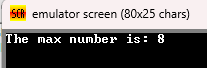
\includegraphics[width = .4\textwidth]{1.png}
    \captionof{figure}{Finding min/max number}
\end{center}


\clearpage
\title{Problem 4.2}
\author{}
\date{}
\maketitle

\section*{Problem Description}
Write a program to display a "?", read two capital letters, and display them on the next line in alphabetical order.

\section*{Process}
\subsection*{Code:}

\begin{multicols}{2}{|}
    \begin{minted}[linenos,breaklines,breakanywhere]{nasm}
DATA SEGMENT
    CR EQU 0DH
    LF EQU 0AH
    MSG1 DB CR, LF, '? $'
    CHAR1 DB ?
    CHAR2 DB ?
DATA ENDS  

CODE SEGMENT
    ASSUME CS:CODE, DS:DATA

START:
    LEA DX, MSG1
    MOV AH, 9
    INT 21H
    
    MOV AH, 1 
    INT 21H
    MOV CHAR1, AL
    
    MOV AH, 1
    INT 21H
    MOV CHAR2, AL
    
    MOV AL, CHAR1
    MOV BL, CHAR2
    
    CMP AL, BL
    JLE SKIP_SWAP
    MOV CHAR1, BL
    MOV CHAR2, AL
    
SKIP_SWAP:
    ; newline
    MOV AH, 2
    MOV DL, 0Dh
    INT 21h
    MOV DL, 0Ah
    INT 21h
    
    ; first character
    MOV AH, 2
    MOV DL, CHAR1
    INT 21h
    
    ; second character
    MOV AH, 2
    MOV DL, CHAR2
    INT 21h
    
    ; Terminate program
    MOV AH, 4Ch
    INT 21h 
    
CODE ENDS

END START
\end{minted}
\end{multicols}

\subsection*{Output}
\begin{center}
    \centering
    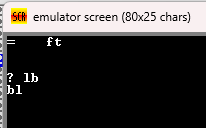
\includegraphics[width = .4\textwidth]{2.png}
    \captionof{figure}{Ordering letters alphabetically}
\end{center}



\clearpage
\title{Problem 4.3}
\author{}
\date{}
\maketitle

\section*{Problem Description}
Write a program that will prompt the user to enter a HEX digit character("0",......"9" or, "A",......"F"), display it on the next line in decimal, and ask the user if he or she wants to do it again. If the user types "Y" or "y", the program terminates. If the user enters an illegal character. prompt the user try again.

\section*{Process}
\subsection*{Code:}

\begin{multicols}{2}{ | }
    \begin{minted}[linenos,breaklines,breakanywhere]{nasm}
DATA SEGMENT
    CR EQU 0DH
    LF EQU 0AH
    MSG1 DB CR, LF, "Enter A HEX Digit: $"
    MSG2 DB CR, LF, "Do it again? $"
    MSG3 DB CR, LF, "In Decimal: $"
    MSG4 DB CR, LF, "In Decimal: 1$"
    MSG5 DB CR, LF, "Try Again.$"
    CHAR DB ?, '$'
    ANS DB ?, '$'
DATA ENDS 

CODE SEGMENT
    ASSUME CS:CODE, DS: DATA
    
START:
    MOV AX, DATA
    MOV DS, AX
    
LOOP_START:
    LEA DX, MSG1
    MOV AH, 9
    INT 21H
    
    MOV AH, 1
    INT 21H
    
    CMP AL, '0'
    JB NOT_NUM
    
    CMP AL, '9'
    JA NOT_NUM
    
    MOV ANS, AL
    
    LEA DX, MSG3
    MOV AH, 9
    INT 21H
    
    MOV DL, ANS
    MOV AH, 2
    INT 21H
    
    JMP LOOP_CHECK
    
NOT_NUM:
    CMP AL, 'A'
    JB ILLEGAL
    
    CMP AL, 'F'
    JA ILLEGAL
    
    MOV ANS, AL
    SUB ANS, 11H
    
    LEA DX, MSG4
    MOV AH, 9
    INT 21H
    
    MOV DL, ANS
    
    MOV AH, 2
    INT 21H
    JMP LOOP_CHECK
    
ILLEGAL:
    LEA DX, MSG5
    MOV AH, 9
    INT 21H
    
LOOP_CHECK:
    LEA DX, MSG2
    MOV AH, 9
    INT 21H
    
    MOV AH, 1
    INT 21H
    
    CMP AL, 'y'
    JZ LOOP_START
    
    CMP AL, 'Y'
    JZ LOOP_START
    
    MOV AH, 4CH
    INT 21H
    
CODE ENDS
END START
\end{minted}
\end{multicols}

\subsection*{Output}
\begin{center}
    \centering
    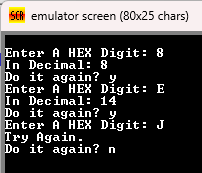
\includegraphics[width = .4\textwidth]{3.png}
    \captionof{figure}{Converting HEX to Decimal}
\end{center}

\clearpage
\title{Problem 4.4}
\author{}
\date{}
\maketitle

\section*{Problem Description}
Write a program to read one of the HEX digits A-F, and display it on the next line in decimal.

\section*{Process}
\subsection*{Code:}

\begin{multicols}{2}{|}
    \begin{minted}[linenos,breaklines,breakanywhere]{nasm}
DATA SEGMENT
    CR EQU 0DH
    LF EQU 0AH
    MSG1 DB CR, LF, "Enter the HEX number : $"
    MSG2 DB CR, LF, "In decimal: 1$"
    NUM DB ?
    DEC_NUM DB ?
DATA ENDS 

CODE SEGMENT
    ASSUME CS:CODE, DS DATA
    
START:
    MOV AX, DATA
    MOV DS, AX
    
    LEA DX, MSG1
    MOV AH, 9
    INT 21H
    
    MOV AH, 1
    INT 21H
    MOV NUM, AL
    
    SUB NUM, 11H
    
    LEA DX, MSG2
    MOV AH, 9
    INT 21H
    
    MOV DL, NUM
    
    MOV AH, 02H
    INT 21H
    
    MOV AH, 4CH
    INT 21H
CODE ENDS
END START
\end{minted}
\end{multicols}

\subsection*{Output}
\begin{center}
    \centering
    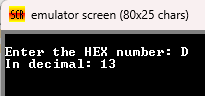
\includegraphics[width = .4\textwidth]{4.png}
    \captionof{figure}{Converting HEX (A-F) to Decimal}
\end{center}

\clearpage
\title{Problem 4.5}
\author{}
\date{}
\maketitle

\section*{Problem Description}

\section*{Process}
\subsection*{Code:}

\begin{multicols}{2}{|}
    \begin{minted}[linenos,breaklines,breakanywhere]{nasm}
DATA SEGMENT
    CR EQU 0DH
    LF EQU 0AH
    STARS DB CR, LF, "**********$"
    COUNTER DW 10
DATA ENDS  

CODE SEGMENT
    ASSUME CS:CODE, DS DATA

START:
    MOV AX, DATA
    MOV DS, AX
    MOV CX, COUNTER
    
LOOP_START:
    LEA DX, STARS
    MOV AH, 9
    INT 21H
    
    DEC CX
    CMP CX, 0 
    
    JE LOOP_END
    JMP LOOP_START 
    
LOOP_END:
    MOV AH, 4CH
    INT 21H 
    
CODE ENDS
END START
    \end{minted}
\end{multicols}

\subsection*{Output}
\begin{center}
    \centering
    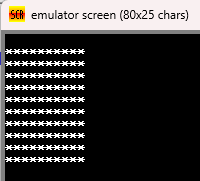
\includegraphics[width = .4\textwidth]{5.png}
    \captionof{figure}{Printing a pattern using Loop}
\end{center}


\section*{Keywords}
These are the new keywords learned while solving the Problems
\begin{description}
    \item[CMP] Used to compare 2 provided byte/word.
    \item[JMP] Used to jump to the provided address to proceed to the next instruction.
    \item[JA] Used to jump if above/not below/equal instruction satisfies.
    \item[JB] Used to jump if below/equal/ not above instruction satisfies.
    \item[JG] Used to jump if greater/not less than/equal instruction satisfies.
    \item[JLE] Used to jump if less than/equal/if not greater than instruction satisfies.
    \item[JZ] Used to jump if equal/zero flag ZF = 1


\end{description}

\end{document}
